\chapter{Introduction}
\section{SimBad project}
The SimBad project (Simulation Birth and Death) is a systems of several applications used in cancer cell proliferation simulations. Cancer cell proliferation simply is a  process of cell growth and division. Abnormal cell proliferation, that is, when  cells that divide only finite amount of time before halting their growth or simply dying start untamed proliferation it may cause cancer development.

The SimBad project is a set of applications developed to simulate such processes. It consists of three primary component - simulation program that runs simulation and generates output stream data - (SimBaD-CLI), simulation output analyzer (SimBaD- analyzer) and plot generator (SimBad-Reports). Components exchange information in pipeline-like way, each component recives some input file (or files) and based on those files it generates some output.

The process of simulation is as follows: it starts with a configuration file in which several dozen objects and parameters that determine the process of simulation. Around ~100 parameter that need to be set and adjusted in order to run simulation. Valid configuration is passed as input to SimBad-CLI which starts the simulation process. The output of CLI step is a .csv file which i turn is input of analyzer step. Form the .csv file, the analyzer step generates multiple .csv and .parquet files, which in turn are necessary to generate plots
in report step.

\begin{figure}[ht]
	\centering
		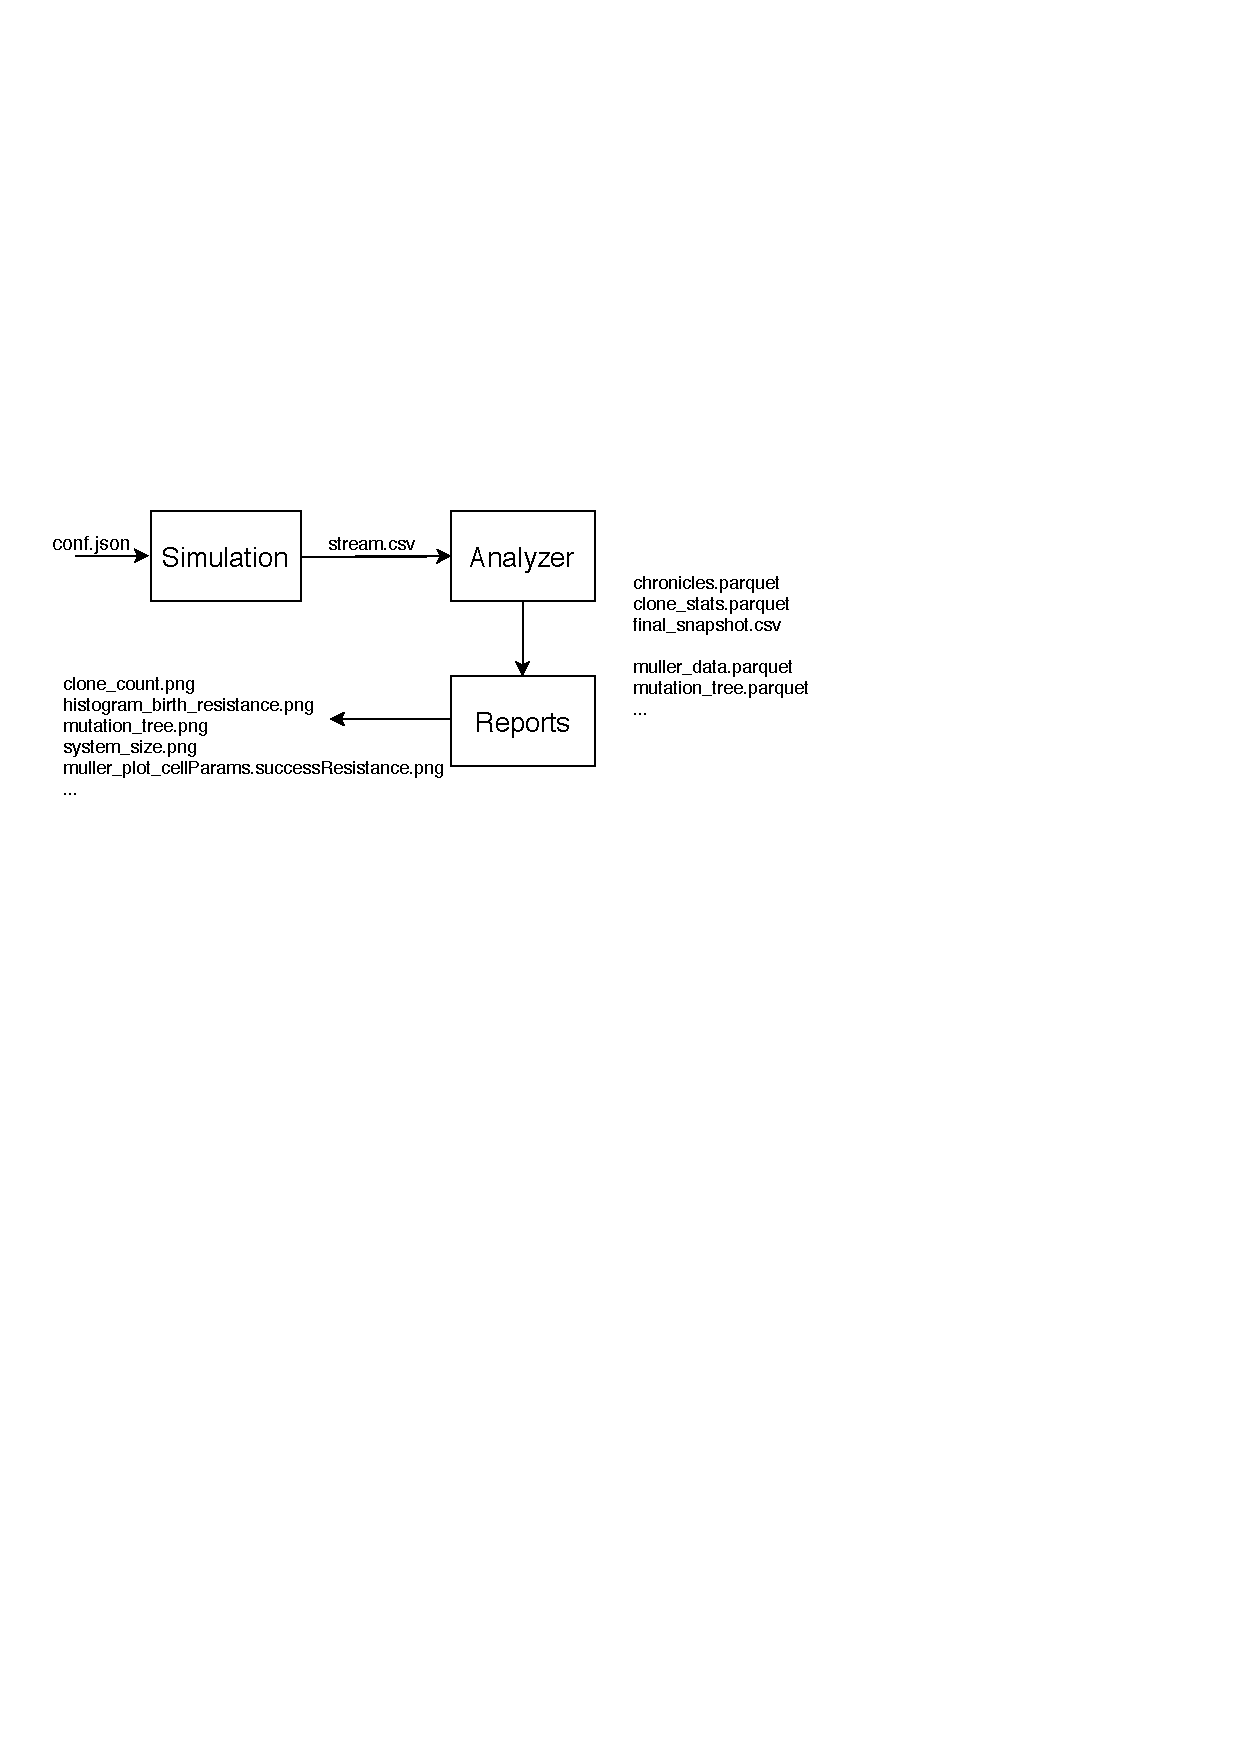
\includegraphics[width=0.9\linewidth]{diagrams/simbad-data-flow.pdf}
	\caption{Data flow between system components}
	\label{fig:data-flow}
\end{figure}

Each step has many dependencies on external libraries that need to be installed on host system and many configuration options that need to be set in order to execute the step. Due to high complexity of system, substantial amount of technical knowledge is needed to run the simulation process, and non-technical user are effectively unable to use this system, without help and guidance of its authors. Moreover, even if the user has required knowledge and skills to install and configure the system, system dependency on third-party code libraries that are not compatible with user machine may prevent the usage of the system.

To enable to users to use this system, an ease to use interface that will allow to control and monitor SimBad simulation process, and ability to install the system in host agnostic way are needed. The purpose of this thesis is to propose and implement such interface. 
Apart of ease of use, several other assumptions were made:
\begin{itemize}
    \item additional system components will be build on top of existing components without modifying them
    \item minimizing the resource footprint on host system
    \item host-agnostic installation
    \item decoupling of components
    \item zero-configuration needed for normal user and extensive configuration available to power user
\end{itemize}
In this thesis I will address each of those assumptions